\section{Взаимодействие с кластером}

В современных задачах зачастую возникают задачи предъявляющие высокие требования к аппаратным мощностям, которые не всегда
могут быть доступны. Зачастую в таком случае прибегают к работе с удаленной машиной, обладающей достаточной вычислительной мощностью,
чтобы удовлетворить требования. Очевидным решением для облегчения взаимодействия конечного пользователя и ПО является клиент-серверное
приложение. Данный подход позволит свести взаимодействие конечного пользователя с исходным кодом программ к минимуму.

В данной работе для работы с серверной частью был использован язык Golang, а в частности пакет \textbf{gin-gonic} \cite{GinGonic}, который является веб-фреймворком,
предоставляющий более быструю работу чем стандартный сетевой пакет. Основной частью пакета является роутер, определяющий
какой запрос пришел со стороны клиента. Разработчик же описывает каким образом должен реагировать сервер на тот или иной запрос, 
путем назначения функций обработчиков на различные варианты запросов. Golang не требует установки какого либо дополнительного программного обеспечения 
для реализации сервера(например Apache), все эти функции уже есть в стандартном сетевом пакете.

Клиентский интерфейс содержит в себе следующие страницы:
\begin{enumerate}
    \item Главная страница
    \item Симуляция системы трех тел
    \item Вычисление двумерного поля энергий
    \item Вычисление трехмерного облака точек
    \item Результаты симуляций
    \item Страница ошибки
\end{enumerate}

Данные страницы реализованы на языке html и формируют GET или POST запросы на сервер. Страницы 2,3,4 -  содержат в себе поля для ввода параметров симуляции 
и интегрирования, которые формируют POST запрос и на сервере, который представляет собой кластер, обрабатываются и запускают симуляцию.  В листинге \ref{lst:post}
реализован парсинг формы запроса, получение даннных, требующихся для запуска симуляции и непосредственно запуск симуляции. 


\begin{lstlisting}[numbers=none, language=Golang,caption=Реализация обработчика POST запроса, label=lst:post]
    r.POST("/sim", func(c *gin.Context) {
		var m [3]float64
		m[0], _ = strconv.ParseFloat(c.PostForm("m1"), 64)
		m[1], _ = strconv.ParseFloat(c.PostForm("m2"), 64)
		m[2], _ = strconv.ParseFloat(c.PostForm("m3"), 64)

		var k [3]float64
		k[0], _ = strconv.ParseFloat(c.PostForm("k1"), 64)
		k[1], _ = strconv.ParseFloat(c.PostForm("k2"), 64)
		k[2], _ = strconv.ParseFloat(c.PostForm("k3"), 64)

		v, _ := strconv.ParseFloat(c.PostForm("vel"), 64)
		l, _ := strconv.ParseFloat(c.PostForm("len"), 64)

		step, _ := strconv.ParseFloat(c.PostForm("stpt"), 64)
		fint, _ := strconv.ParseFloat(c.PostForm("fint"), 64)

		c.Redirect(301, "/dat")
		avg := c.Request.FormValue("avg")

		body := slv.NewThreeBodyModel(m, k)
		//y, mon, d := time.Now().Date()
		filename := fmt.Sprintf("sym%v.dat", time.Now().Format("15:04:05_02Jan06"))
		file, err := os.Create(fmt.Sprint("./dat/", filename))
		if err != nil {
			log.Println("Cannot create file!  :", err)
			c.File("./www/error.html")
			return
		}

		machine := slv.StateMachFromModel(body, v, l, step, 0, fint)
		if avg == "on" {
			go func(machine grn.StateMachine, body grn.ThreeBodyModel, file *os.File, filename string) {
				filsys[filename] = false
				slv.SimulateAv(machine, body, file)
				filsys[filename] = true
			}(machine, body, file, filename)

		} else {
			go func(machine grn.StateMachine, file *os.File, filename string) {
				filsys[filename] = false
				time.Sleep(30 * time.Second)
				slv.Simulate(machine, file)
				filsys[filename] = true
			}(machine, file, filename)
		}
	})
\end{lstlisting}

Симуляция запускается отдельной горутиной, что позволяет работать серверу и расчетному ПО параллельно и не останавливать работу сервера. Также для реализации 
отслеживания процесса расчетов был реализован ассоциативный массив \textit{filsys}, который содержит текущее состояние для каждого файла симуляции, где имя файла является ключом, 
а значение отображает состояние файла, если значение \textit{false}, то вычисление данного файла еще не закончено, иначе файл может быть загружен с кластера для дальнейшей 
визуализации.

Страница 5, формируется динамически сервером, в зависимости от состояния файла \textit{filsys}. Для автоматической генерации html страницы используется 
пакет \textit{template}, который позволяет формировать страницу в зависимости от контекста.

\begin{lstlisting}[numbers=none, language=html,caption=Html шаблон, label=lst:templ]
    <!DOCTYPE html>
    <html>
    <head>
        <meta charset="UTF-8" />
    </head>
    <body>
        <div>
            <p><h2>Simulation results</h1></p>
            <hr>
            {{ range $key, $value := . }}
                <li>
                    {{ $key }}
                    {{if $value }}
                        <form method="POST" action="/dat">
                            <input name="file" type="hidden" value="{{ $key }}"><input type="submit"  value="Download">
                        </form>
                    {{else}}
                        <strong>File in progress...</strong>
                    {{end}}
                </li>
            {{ end }}
        </div>
        <a href="/">Back to menu</a>
    </body>
    </html>
\end{lstlisting}

Шаблон в листинге \ref{lst:templ}, формирует страницу в зависимости от значений \textit{filesys}, \textit{range  \$key, \$value := . } - цикл, 
который перебирает все ключи и значения, переданные программой, формирующей страницу(листинг \ref{lst:frm}). В зависимости от значений \textit{\$value}, формируется либо сообщение
о том что файл еще рассчитывается, либо форма POST запроса со скрытым полем, содержащим имя файла. При нажатии на кнопку выбранный файл расчетов скачивается
с кластера на клиентскую машину.

\begin{lstlisting}[numbers=none, language=html,caption=Формирование html, label=lst:frm]
r.GET("/dat", func(c *gin.Context) {
		t, err := template.ParseFiles("./www/dat.html")
		if err != nil {
			panic(err)
		}

		err = t.Execute(c.Writer, filsys)
		if err != nil {
			panic(err)
		}
    })
\end{lstlisting}

\newpage
\begin{figure}[h]
    \centering
    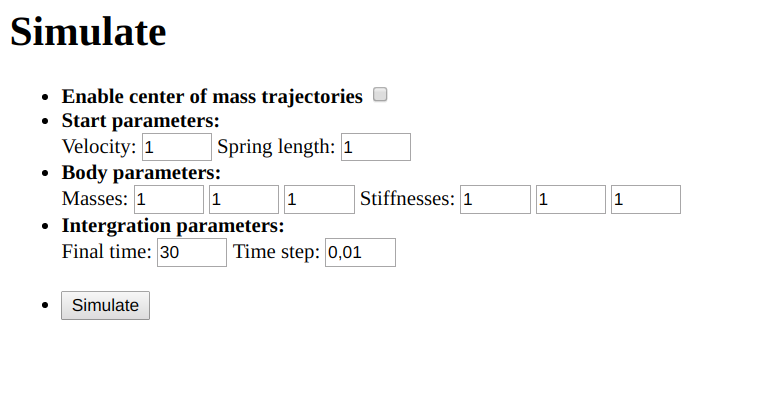
\includegraphics[width=0.7\textwidth]{net/scren1.png}
    \caption{Зависимость $\Delta \tilde{E}$ от различных значений масс. Каждый график соответствует одной переменной массе.}
\end{figure}

\newpage
\begin{figure}[h]
    \centering
    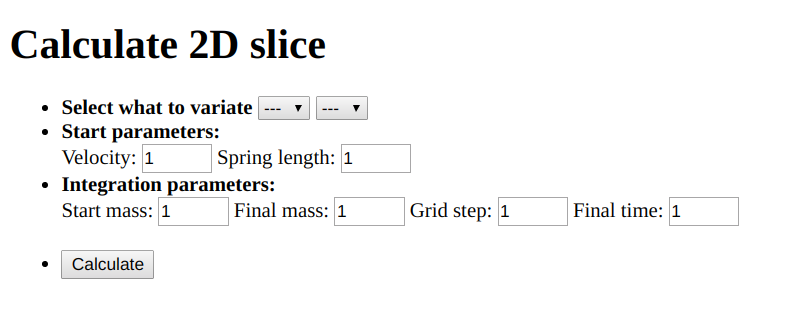
\includegraphics[width=0.7\textwidth]{net/scren2.png}
    \caption{Зависимость $\Delta \tilde{E}$ от различных значений масс. Каждый график соответствует одной переменной массе.}
\end{figure}

\newpage

\begin{figure}[h]
    \centering
    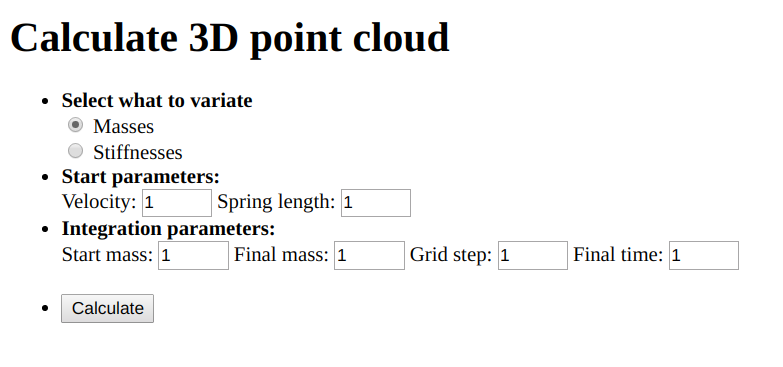
\includegraphics[width=0.7\textwidth]{net/scren3.png}	
    \caption{Зависимость $\Delta \tilde{E}$ от различных значений масс. Каждый график соответствует одной переменной массе.}
\end{figure}
